\begin{flushright} {\tiny {\color{gray} (tikz\_quadrature\_rectangle.tex)}} \end{flushright}
%~~~~~~~~~~~~~~~~~~~~~~~~~~~~~~~~~~~~~~~~~~~~~~~~~~~~~~~~~~~~~~~~~~~~~~~~~~~~~~~~~~~~~~~~~~~~~~~~~~

\begin{center}
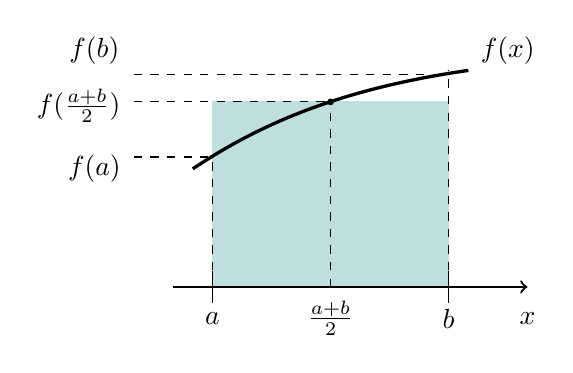
\begin{tikzpicture}
%\draw[step=0.5cm,gray,very thin] (0,0) grid (7,5); 
\draw[fill=teal!25,teal!25](1,1) rectangle (4,3.35);
\draw [thick, ->] (0.5,1) -- (5,1);
\node[] at (1,0.6) {$a$};
\node[] at (4,0.6) {$b$};
\node[] at (5,0.6) {$x$};
\node[] at (2.5,0.6) {$\frac{a+b}{2}$};
\draw [-] (1,0.8) -- (1,1.2);
\draw [-] (4,0.8) -- (4,1.2);
\draw [dashed] (1,1) -- (1,2.6);
\draw [dashed] (2.5,1) -- (2.5,3.35);
\draw [dashed] (4,1) -- (4,3.75);
\draw[black,fill=black] (2.5,3.35)   circle (1pt);
\draw[very thick] (0.75,2.5) .. controls (1.5,3) and (2.5,3.5) .. (4.25,3.75);
\node[] at (4.75,4) {$f(x)$};
\node[] at (-0.7,3.3) {$f(\frac{a+b}{2})$};
\draw [dashed] (0,3.35) -- (2.5,3.35);
\node[] at (-0.5,2.5) {$f(a)$};
\draw [dashed] (0,2.65) -- (1,2.65);
\node[] at (-0.5,4) {$f(b)$};
\draw [dashed] (0,3.7) -- (4,3.7);
\end{tikzpicture}
\end{center}

